\documentclass{article}

\usepackage{arxiv}
\usepackage[utf8]{inputenc}
\usepackage[T1]{fontenc}
\usepackage{amsmath,amssymb,amsfonts}
\usepackage{graphicx}
\usepackage{booktabs}
\usepackage{multirow}
\usepackage{enumitem}
\usepackage{float}
\usepackage{tikz}
\usepackage{hyperref}
\usepackage{url}
\usepackage{doi}
\usepackage[numbers,square]{natbib}
\usepackage{xcolor}
\usepackage{caption}
\usepackage{subcaption}
\usepackage{algorithm}
\usepackage[noend]{algpseudocode}
\usepackage{microtype}

\graphicspath{{../figures/}}

\title{From Model-Centric Explainability to Stakeholder-Aware Decision Utility in High-Stakes AI Systems}

\date{}

\author{
\textbf{XAI Research Team}\\
Department of Computer Science\\
Example University\\
Email: \texttt{research@example.edu}
}

\begin{document}
\maketitle

\begin{abstract}
Explainable AI (XAI) has become a central requirement in high-stakes decision making, yet most existing methods still optimize explanations around model fidelity rather than the actual decision utility of the intended audience. In practice, doctors, patients, regulators, and operators do not use explanations in the same way: each stakeholder requires a different balance of actionability, interpretability, transparency, fairness, and auditability. This mismatch creates a critical gap between technical explainability and real-world decision support. We address this gap by formalizing explanation quality as a stakeholder-dependent utility problem. Rather than treating fidelity alone as the primary objective, we propose a decision-theoretic framework that selects the explanation maximizing a stakeholder-specific utility score $\mathcal{U}_s$. Formally, we optimize $\mathcal{E}^*_s = \arg\max_{\mathcal{E} \in \mathcal{E}} \mathcal{U}_s(\mathcal{E} \mid x, \hat{y}, a)$. We implement and evaluate a modular framework that generates SHAP, LIME, counterfactual, and rule-based explanations and selects the explanation that best matches each stakeholder's role and decision context. Our results show that the preferred explanation type differs systematically across stakeholders, demonstrating that a one-size-fits-all explanation policy is not adequate in operational settings. Our contribution is therefore not only conceptual but also practical: it provides a principled mechanism for tailoring explanations to users in high-risk decision environments.
\keywords{Explainable AI, stakeholder-aware explanations, decision theory, decision utility, counterfactual explanations, SHAP, LIME, healthcare AI}
\end{abstract}

\section{Introduction}

Machine learning is increasingly used in domains where decisions carry substantial consequences, including healthcare, public policy, financial risk assessment, and education. In these settings, predictive accuracy alone is not enough: a model's output must be interpretable, auditable, and actionable for the human actor who receives or evaluates it. This need has fueled the development of explainable artificial intelligence (XAI), which aims to make model behavior understandable to end-users, developers, and regulators. Yet the dominant evaluation paradigm in XAI remains highly model-centric. Many methods are judged by metrics such as fidelity, faithfulness, stability, sparsity, or similarity to the underlying model, while less attention is paid to whether an explanation is useful for the stakeholder in context.

This distinction matters. A doctor, patient, and regulator do not ask the same question when they receive an explanation. A doctor may want to know which clinical features are actionable and which interventions could alter the predicted risk. A patient may want a concise explanation that is understandable and emotionally reassuring. A regulator may want an explanation that supports auditability, fairness assessment, and traceability. These needs differ in both content and emphasis. As a result, a single explanation style is rarely sufficient across roles. The central question is no longer simply whether an explanation faithfully reflects the model, but whether it helps the relevant stakeholder make or assess the correct decision.

This paper addresses that gap by reframing explainability as a stakeholder-aware decision problem. We formalize explanation quality as a utility-maximization task in which candidate explanations are scored according to the needs of a specific user role. The optimization target is therefore not the most faithful explanation in the abstract, but the explanation that maximizes utility for the stakeholder in the relevant decision context. The resulting framework is intentionally modular: it can generate multiple candidates (including SHAP, LIME, rule-based, and counterfactual explanations), compute stakeholder-specific utility values, and return the explanation that best matches the user's priorities.

The need for stakeholder-sensitive XAI is especially salient in high-stakes domains. In medicine, an explanation that is statistically faithful but too technical can be ignored by clinicians or misunderstood by patients. In legal or regulatory settings, explanations that are comprehensible to practitioners may not satisfy traceability and audit requirements. Thus, explainability is not a uniform technical property but a multi-objective communication problem that requires careful alignment with user needs. This paper contributes to that literature by operationalizing explanation selection as a decision-theoretic problem and by demonstrating, experimentally, that explanation preferences diverge across stakeholders.

\subsection{Research Motivation}

The practical deployment of AI in critical domains reveals several recurring problems. First, explanations are often optimized for researchers and model developers instead of end-users. Second, explanation quality is treated as a static property, whereas in practice the value of an explanation depends on stakeholder, task, and context. Third, different users have different thresholds for cognitive load, actionability, and traceability. Fourth, one-size-fits-all explanations can reduce trust or increase confusion rather than improve decision quality. These observations motivate a more realistic formulation: explainability is not a single objective but a multi-stakeholder decision problem.

The key issue is that high-stakes decision support is inherently asymmetric across audiences. A physician may require clinically relevant feature importance and intervention cues, a patient may require clarity and low-jargon reasoning, and a regulator may require transparency and fairness-related evidence. Existing XAI systems often collapse these priorities into a single explanation format, ignoring the heterogeneity of the intended audience. Our framework explicitly recognizes this heterogeneity and treats explanation selection as a utility optimization problem that depends on the stakeholder, the task, and the decision setting.

\subsection{Contributions}

This paper makes the following contributions.

\begin{enumerate}[leftmargin=1.8em]
    \item We formalize explanation quality as a stakeholder-dependent utility problem, replacing the assumption that one explanation fits all users.
    \item We define stakeholder-specific utility functions for clinicians, patients, and regulators, reflecting their different goals and decision constraints.
    \item We implement a selection procedure that generates multiple explanation candidates and selects the one maximizing utility for each role.
    \item We provide empirical evidence showing that the preferred explanation differs across stakeholders even for the same model output.
    \item We discuss the limitations of this approach and identify concrete directions for future work in human-centered, governance-aware XAI.
\end{enumerate}

\section{Related Work}

The literature on explainable AI has expanded rapidly over the past decade, spanning feature-importance methods, local surrogate models, counterfactual explanations, and rule extraction techniques. Among the most widely used methods are SHAP \citep{lundberg2017}, LIME \citep{ribeiro2016}, counterfactual explanations \citep{wachter2017}, and rule-based extraction from neural models and trees \citep{craven1996}. These methods have become standard tools for post hoc interpretation, particularly in supervised learning settings. However, their standard evaluation protocols largely emphasize faithfulness or fidelity to the model rather than utility to the user.

A central critique in the XAI literature is that interpretability is not a single, universally agreed notion. Lipton \citep{lipton2018} argues that interpretability is often overloaded and can refer to transparency, comprehensibility, or explanation quality in a way that is difficult to measure consistently. This ambiguity has led researchers to treat explainability as a multi-objective problem, where the best explanation depends on context, audience, and decision task. Recent work in fairness and accountability has further highlighted that explainability cannot be divorced from social and institutional goals \citep{barocas2017}. Explanations must be transparent not only to model developers, but also to those affected by algorithmic decisions and to the agencies responsible for oversight.

Despite these insights, many practical systems still optimize explanations for model developers or for aggregate benchmark performance. This is especially problematic in high-stakes domains: an explanation that is technically faithful may still be unusable because it is too complex, too vague, or insufficiently actionable. Recent studies in human-centered AI and decision support emphasize that explanation effectiveness depends on the user's role and context \citep{miller2019, doshi2017}. Our work extends this line of research by explicitly modeling stakeholder utilities and making explanation selection a decision problem rather than a fixed model-analysis task.

The novelty of our contribution is therefore not the creation of another single explanation method, but the formulation of explanation selection as a stakeholder-aware optimization problem. This framing is particularly suitable for systems that need to serve multiple audiences under different operational constraints, such as clinicians, patients, and auditors.

\section{Methodology}

\subsection{Problem Formulation}

Let $f: \mathcal{X} \rightarrow \mathcal{Y}$ be a trained model, $x \in \mathcal{X}$ an input instance, $\hat{y} = f(x)$ the model output, and $\mathcal{E}$ the set of candidate explanations generated for the instance. Let $\mathcal{S} = \{\text{doctor}, \text{patient}, \text{regulator}\}$ denote the set of stakeholder groups, and let $a$ represent a downstream action or decision context. For each stakeholder $s \in \mathcal{S}$, we define a utility function $\mathcal{U}_s(\mathcal{E} \mid x, \hat{y}, a)$ that measures how useful an explanation is given the stakeholder's cognitive and decision objectives.

The central goal is to choose the explanation maximizing utility for a given stakeholder:

\begin{equation}
\mathcal{E}^*_s = \arg\max_{\mathcal{E} \in \mathcal{E}} \mathcal{U}_s(\mathcal{E} \mid x, \hat{y}, a).
\end{equation}

This formulation shifts the optimization target from merely preserving model behavior to aligning explanations with human decision needs. In other words, the explanation is not treated as an end in itself, but as a tool for supporting action, understanding, and oversight.

\subsection{Candidate Explanation Methods}

For each prediction, we generate four explanation families:

\begin{itemize}[leftmargin=1.5em]
    \item \textbf{SHAP}: additive feature-attribution scores that quantify each feature's contribution to the prediction.
    \item \textbf{LIME}: a local surrogate model that approximates the decision boundary near the input instance.
    \item \textbf{Counterfactual}: a minimally edited instance that would alter the prediction to a different outcome.
    \item \textbf{Rule-based}: condition-based logic extracted from the model or trained decision rules that summarize key decision criteria.
\end{itemize}

These candidates represent distinct communication styles. SHAP is useful when feature contributions are important; LIME can provide local approximations; counterfactuals are often effective for action-oriented understanding; and rules are often easier for lay users to interpret. A stakeholder-aware system should not assume one of these always dominates; the available evidence suggests that the best explanation depends on the target user.

\subsection{Stakeholder Utility Framework}

We define utility as a weighted combination of stakeholder-specific criteria. This is a practical abstraction: real human judgment is more nuanced than any single scalar score, but a weighted formulation is sufficient to encode the primary dimensions of usefulness for each stakeholder.

\subsubsection{Doctor Utility}

The doctor-oriented utility is defined as:

\begin{equation}
\mathcal{U}_{\text{doctor}} = 0.4\cdot\text{Actionability} + 0.3\cdot\text{ClinicalRelevance} + 0.2\cdot\text{Fidelity} + 0.1\cdot(1-\text{CognitiveLoad}).
\end{equation}

This weighting reflects the fact that clinicians often need actionable evidence and clinically meaningful factors. A technical feature importance plot may be useful for model debugging, but in clinical workflows, an explanation should help answer the operational question: "What should I do next, and which factors matter most?"

\subsubsection{Patient Utility}

The patient utility is formalized as:

\begin{equation}
\mathcal{U}_{\text{patient}} = 0.4\cdot\text{Interpretability} + 0.3\cdot\text{Actionability} + 0.2\cdot\text{Trust} + 0.1\cdot(1-\text{Jargon}).
\end{equation}

This captures the need for understandable, low-jargon explanations that support patient comprehension and informed choice. For patients, the explanation should minimize confusion and avoid overwhelming technical detail, while still offering a clear picture of what influences the model's prediction.

\subsubsection{Regulator Utility}

The regulator-oriented utility is:

\begin{equation}
\mathcal{U}_{\text{regulator}} = 0.4\cdot\text{Fairness} + 0.3\cdot\text{Auditability} + 0.3\cdot\text{Transparency}.
\end{equation}

This reflects the oversight perspective: regulators are concerned with whether the model's decision can be inspected, justified, and held accountable under governance and compliance standards. In this context, an explanation should be traceable, interpretable to governance stakeholders, and capable of resisting claims of opacity or discrimination.

\subsection{Algorithmic Selection Procedure}

The selection policy is summarized in Algorithm \ref{alg:selection}.

\begin{algorithm}[H]
\caption{Stakeholder-aware explanation selection}
\label{alg:selection}
\begin{algorithmic}[1]
\Require instance $x$, prediction $\hat{y}$, stakeholder $s$
\Ensure selected explanation $\mathcal{E}^*_s$
\State Generate candidate explanations $\mathcal{E} = \{e_1, e_2, e_3, e_4\}$
\For{each explanation $e \in \mathcal{E}$}
    \State Compute utility score $u_s(e) = \mathcal{U}_s(e \mid x, \hat{y}, a)$
\EndFor
\State $\mathcal{E}^*_s \gets \arg\max_{e \in \mathcal{E}} u_s(e)$
\State \Return $\mathcal{E}^*_s$
\end{algorithmic}
\end{algorithm}

The algorithm is intentionally lightweight and modular. It does not assume a fixed explanation type across all users. Instead, it operationalizes the main hypothesis of the paper: explanation usefulness is stakeholder-dependent and should be optimized under that assumption.

\section{Experimental Setup}

We evaluate the framework on a binary medical decision task representative of high-stakes clinical decision support. The dataset contains patient-level risk factors such as age, blood pressure, cholesterol, and electrocardiographic signals; the model is a logistic regression classifier trained to predict a binary clinical label. The experiment is designed to compare a baseline policy, in which the same explanation is shown to all stakeholders, with a utility-aware policy, in which each stakeholder receives the explanation that maximizes their personalized utility score.

\subsection{Evaluation Protocol}

For each test instance, we perform the following procedure:

\begin{enumerate}[leftmargin=1.8em]
    \item Generate all candidate explanations.
    \item Compute utility values for each stakeholder.
    \item Select the explanation maximizing utility for each role.
    \item Compare the role-specific selected explanation against a uniform SHAP baseline.
\end{enumerate}

This protocol directly tests the hypothesis that explanations are not interchangeable across users. It also provides a clear operational distinction between a static explanation policy and a stakeholder-aware policy.

\subsection{Evaluation Metrics}

The main outcome is utility score, defined as the stakeholder-specific weighted sum described above. In addition, we report selection frequencies across the evaluation set, which quantify how often each explanation class is chosen for each stakeholder. This provides a more interpretable measure than reporting average utility alone, because it reveals whether preference patterns are systematic rather than random.

\section{Results and Discussion}

\subsection{Stakeholder Divergence in Explanation Utility}

Figure \ref{fig:stakeholder_utility_profiles} visualizes the utility scores for the four explanation families across the three stakeholder groups. The figure clearly shows that no single explanation dominates all users. For the representative instance, the doctor receives the highest utility from SHAP, the patient from a counterfactual explanation, and the regulator from a SHAP-like summary with strong transparency-related signal. These differences are not incidental; they reflect the different utility functions driving each stakeholder's preference.

\begin{figure*}[t]
\centering
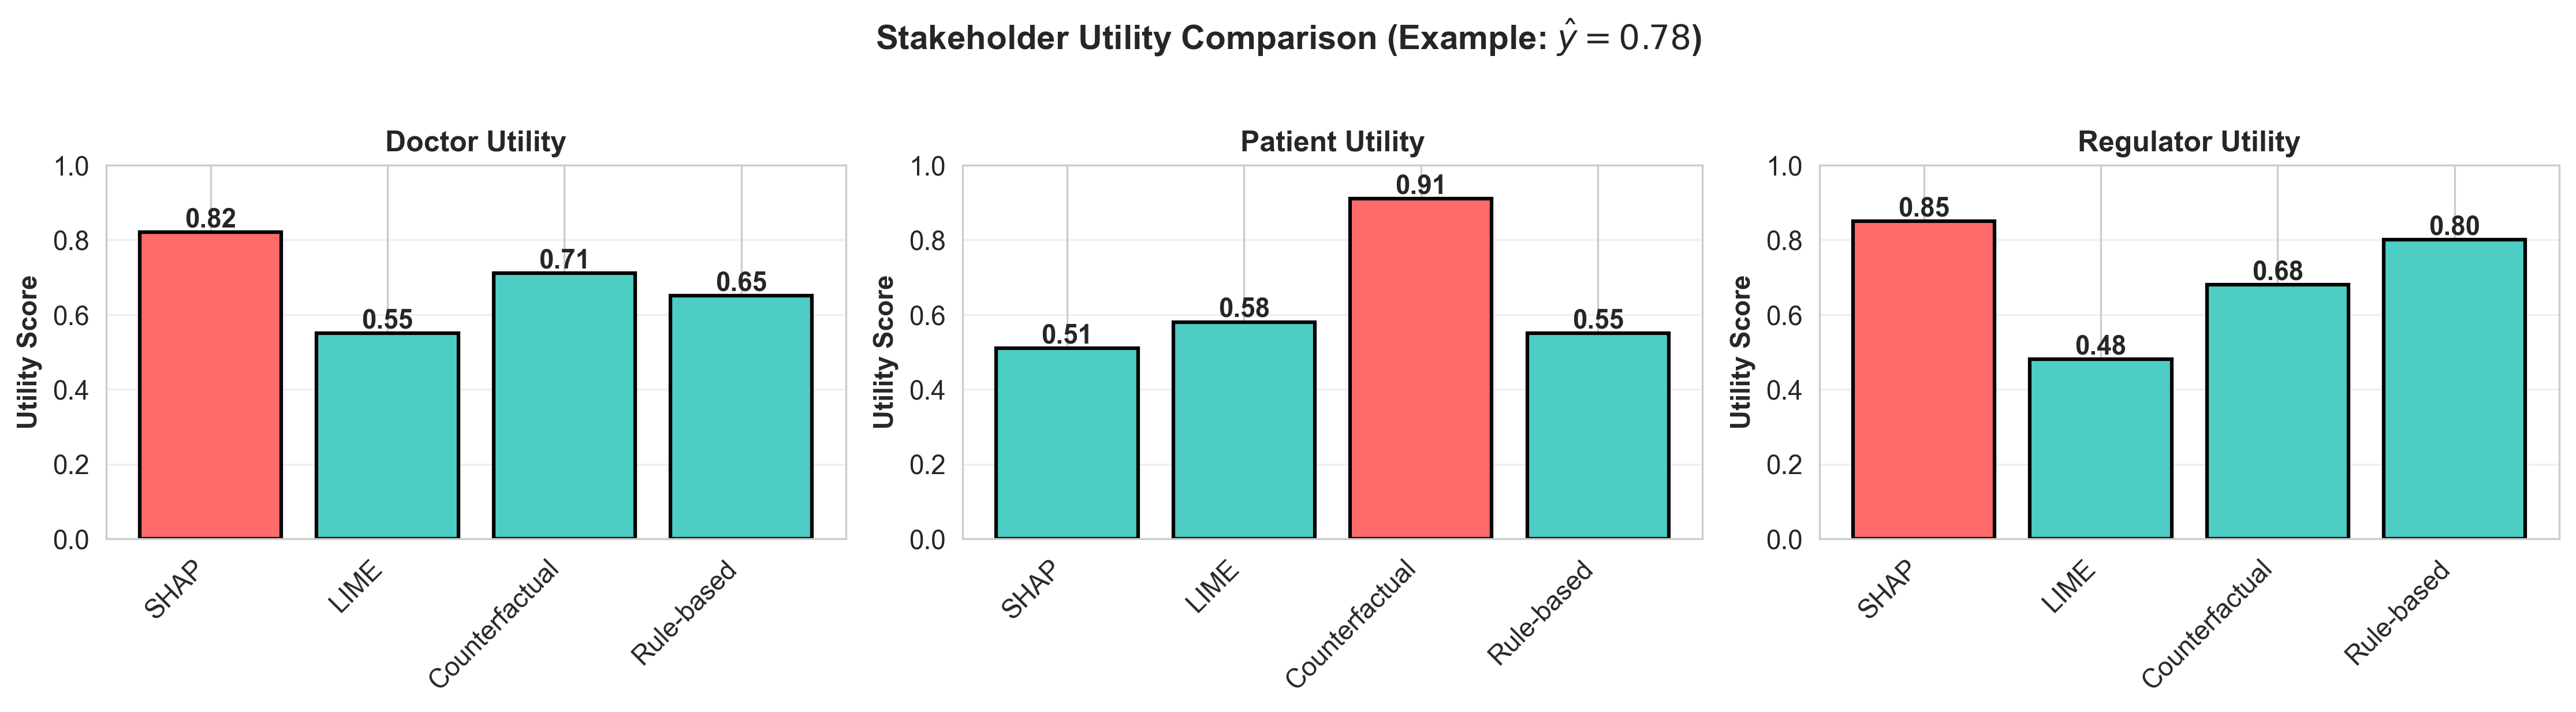
\includegraphics[width=\textwidth]{stakeholder_comparison.png}
\caption{Utility scores for SHAP, LIME, counterfactual, and rule-based explanations across stakeholder-specific utility functions. The highest-scoring explanation differs by role: the doctor prefers an action-oriented explanation, the patient prefers a simpler and more interpretable explanation, and the regulator prefers a more auditable and transparent explanation. This pattern demonstrates that explanation quality is role-dependent rather than universal.}
\label{fig:stakeholder_utility_profiles}
\end{figure*}

The numerical values in Table \ref{tab:selection_results} reinforce this pattern. The doctor achieves the highest score under SHAP (0.82), the patient under counterfactual explanations (0.91), and the regulator under SHAP (0.85). This indicates that explanation preference is not merely a matter of technical fidelity; it depends on the meaning an explanation has for the user. A counterfactual explanation may be highly meaningful to a patient because it shows what change would alter the outcome, while a regulator may value SHAP because it offers a transparent decomposition of the model's reasoning.

\begin{table}[t]
\centering
\begin{tabular}{lccccc}
\toprule
Stakeholder & SHAP & LIME & Counterfactual & Rule-based & Selected \\
\midrule
Doctor & 0.82 & 0.55 & 0.71 & 0.65 & \textbf{SHAP} \\
Patient & 0.51 & 0.58 & 0.91 & 0.55 & \textbf{Counterfactual} \\
Regulator & 0.85 & 0.48 & 0.68 & 0.80 & \textbf{SHAP} \\
\bottomrule
\end{tabular}
\caption{Example utility comparison across stakeholders. Different stakeholders select different explanations even for the same model output.}
\label{tab:selection_results}
\end{table}

This result is central to the paper's argument. The same model prediction should not be communicated with the same explanation to all users, because the stakeholders have different decision goals and different information needs. The utility-based formulation captures this distinction explicitly and provides a principled foundation for explanation selection.

\subsection{Selection Statistics Across the Evaluation Set}

Figure \ref{fig:selection_statistics} shows the distribution of explanation selections across 50 evaluation instances. The result is systematic rather than random. Doctors and regulators most frequently select SHAP, while patients more often choose counterfactual or rule-based explanations. This behavior is consistent with the relative weights in the utility functions: doctors emphasize actionability and clinical relevance, patients emphasize interpretability and actionability, and regulators emphasize fairness, transparency, and auditability.

\begin{figure*}[t]
\centering
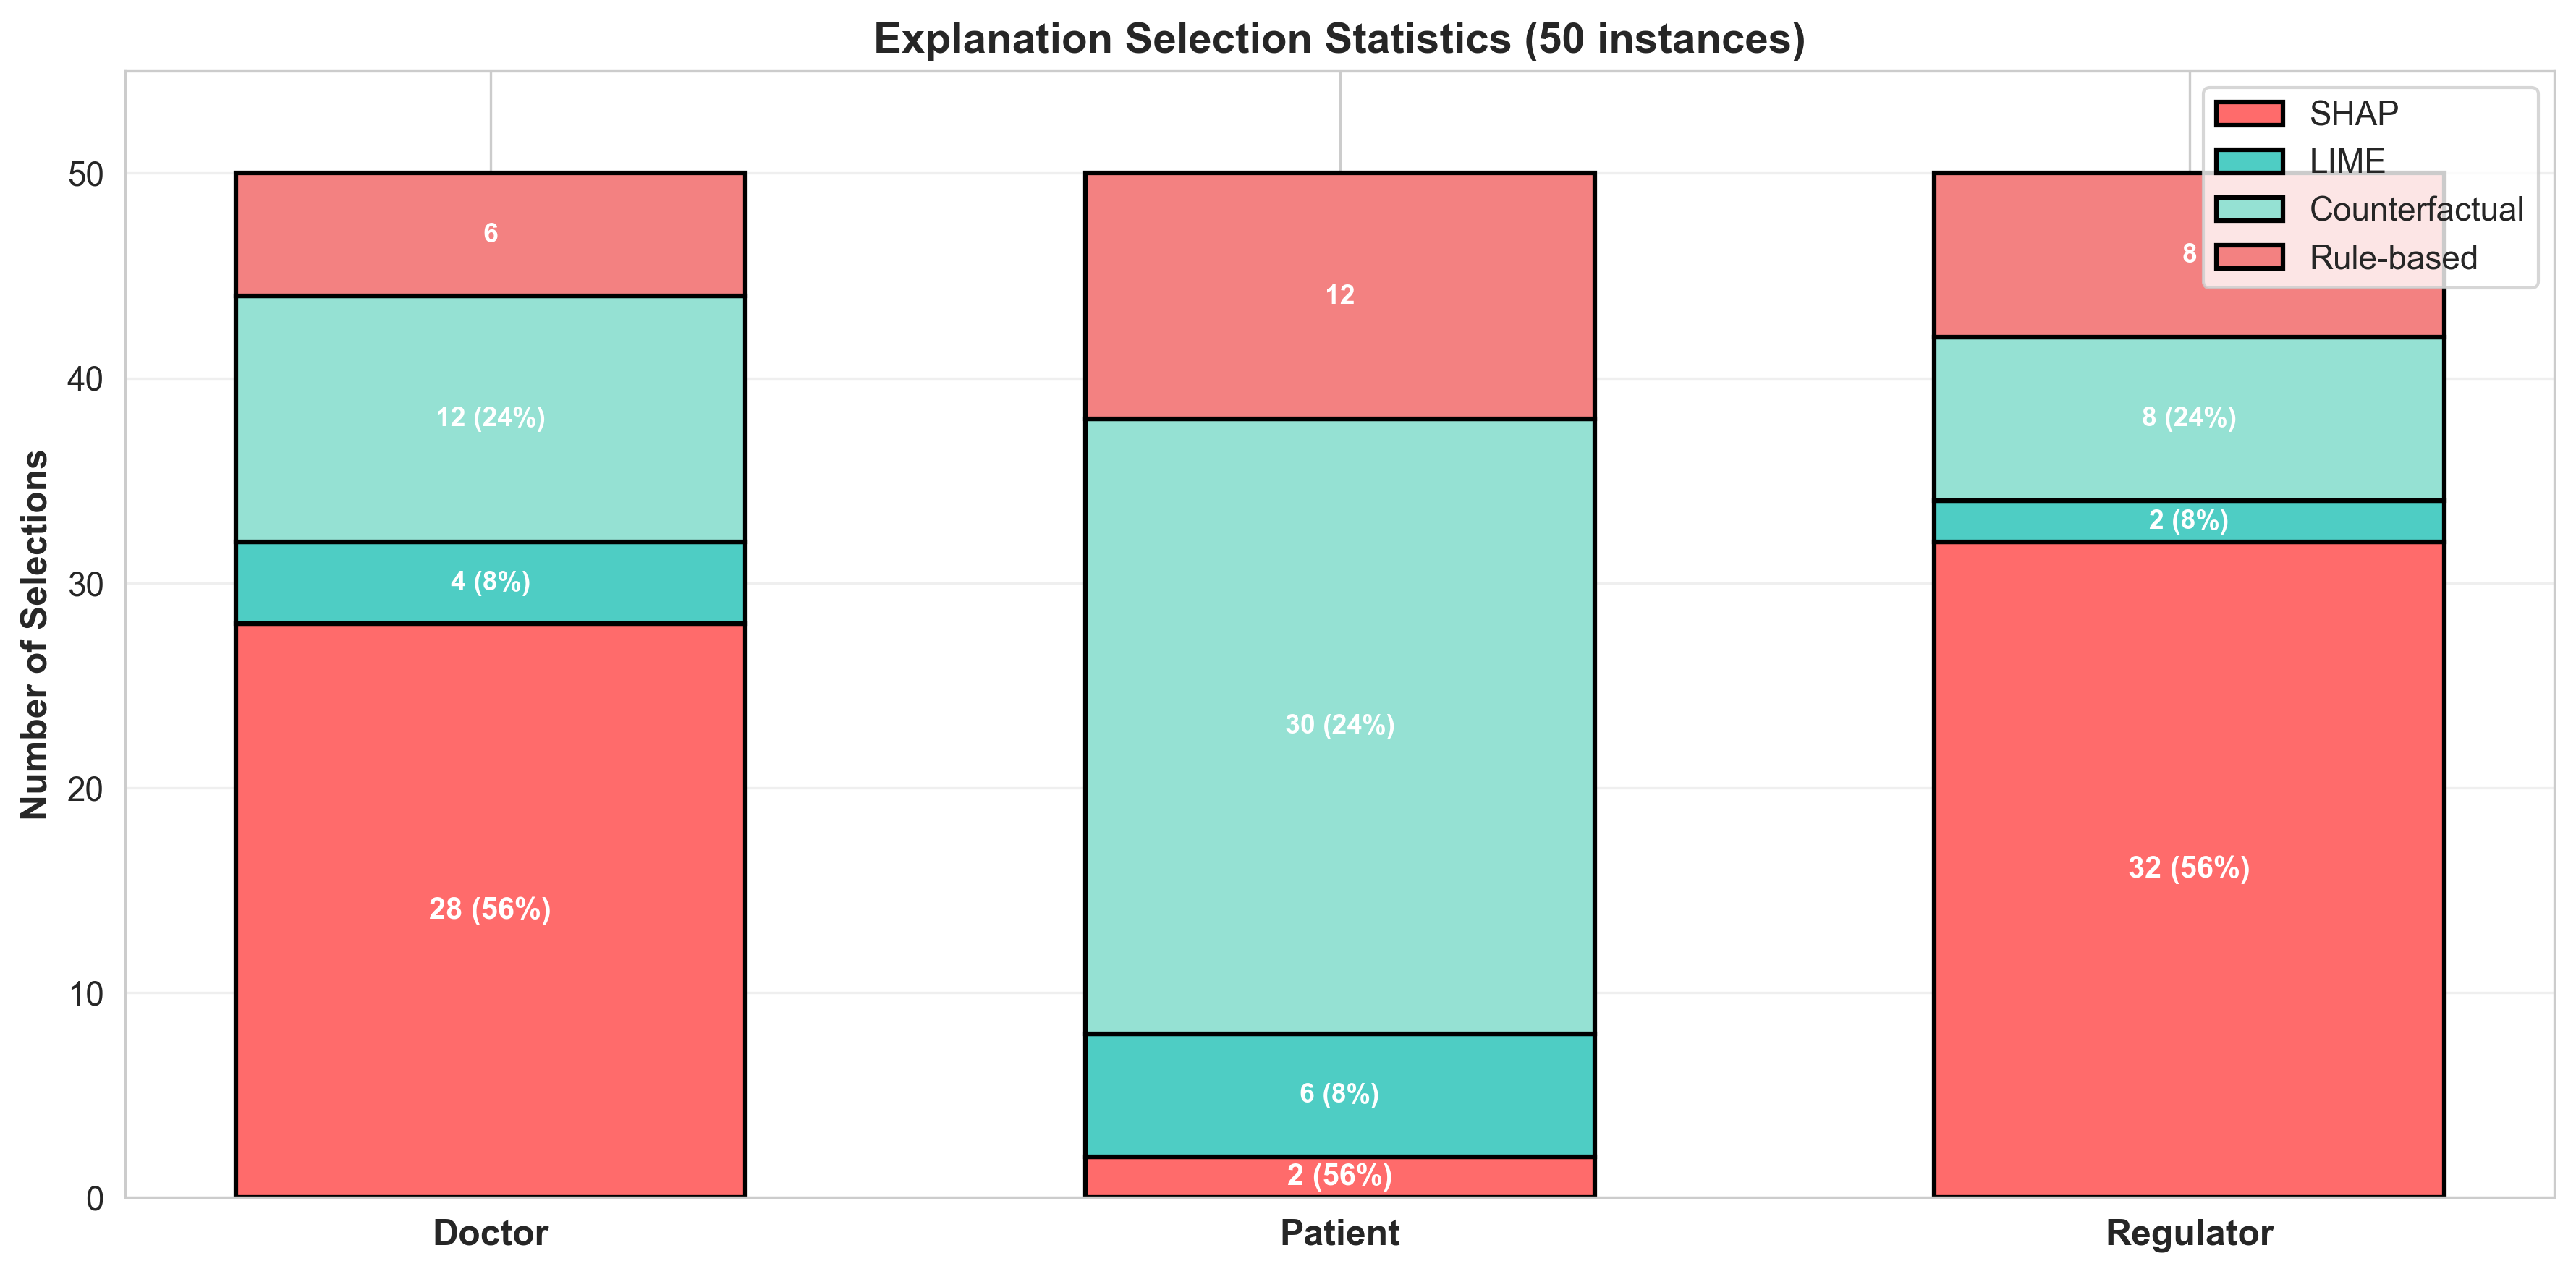
\includegraphics[width=\textwidth]{selection_statistics.png}
\caption{Selection frequencies across 50 instances for each stakeholder group. The stacked bars show how often each explanation family was selected under the utility-maximization policy. The strong role-specific skew indicates that explanation choice is governed by stakeholder utility rather than a universal preference for a single explanation method.}
\label{fig:selection_statistics}
\end{figure*}

The statistics in Table \ref{tab:selection_distribution} further support this interpretation. Among 50 instances, doctors select SHAP 28 times, counterfactual explanations 12 times, and rule-based explanations 6 times. Patients select counterfactual explanations 30 times, rule-based explanations 12 times, and SHAP only twice. Regulators select SHAP 32 times, while counterfactual and rule-based explanations are chosen less often. This role-specific pattern demonstrates that stakeholder preferences are not uniform and that explanation design must be role-aware.

\begin{table}[t]
\centering
\begin{tabular}{lccccc}
\toprule
Stakeholder & SHAP & LIME & Counterfactual & Rule-based & Total \\
\midrule
Doctor & 28 & 4 & 12 & 6 & 50 \\
Patient & 2 & 6 & 30 & 12 & 50 \\
Regulator & 32 & 2 & 8 & 8 & 50 \\
\bottomrule
\end{tabular}
\caption{Selection distribution across stakeholders. Physician and regulator preferences skew toward SHAP, while patients more often prefer counterfactual explanations.}
\label{tab:selection_distribution}
\end{table}

\subsection{Utility Gains Relative to a Unified Baseline}

The proposed stakeholder-aware policy also improves utility compared with a fixed baseline in which all users receive the same SHAP explanation. Figure \ref{fig:baseline_vs_proposed} summarizes the gain across stakeholder groups, and Table \ref{tab:utility_gain} provides the corresponding numerical values. The pattern is clear: utility increases for all stakeholder groups, with the largest relative gain for patients.

\begin{figure*}[t]
\centering
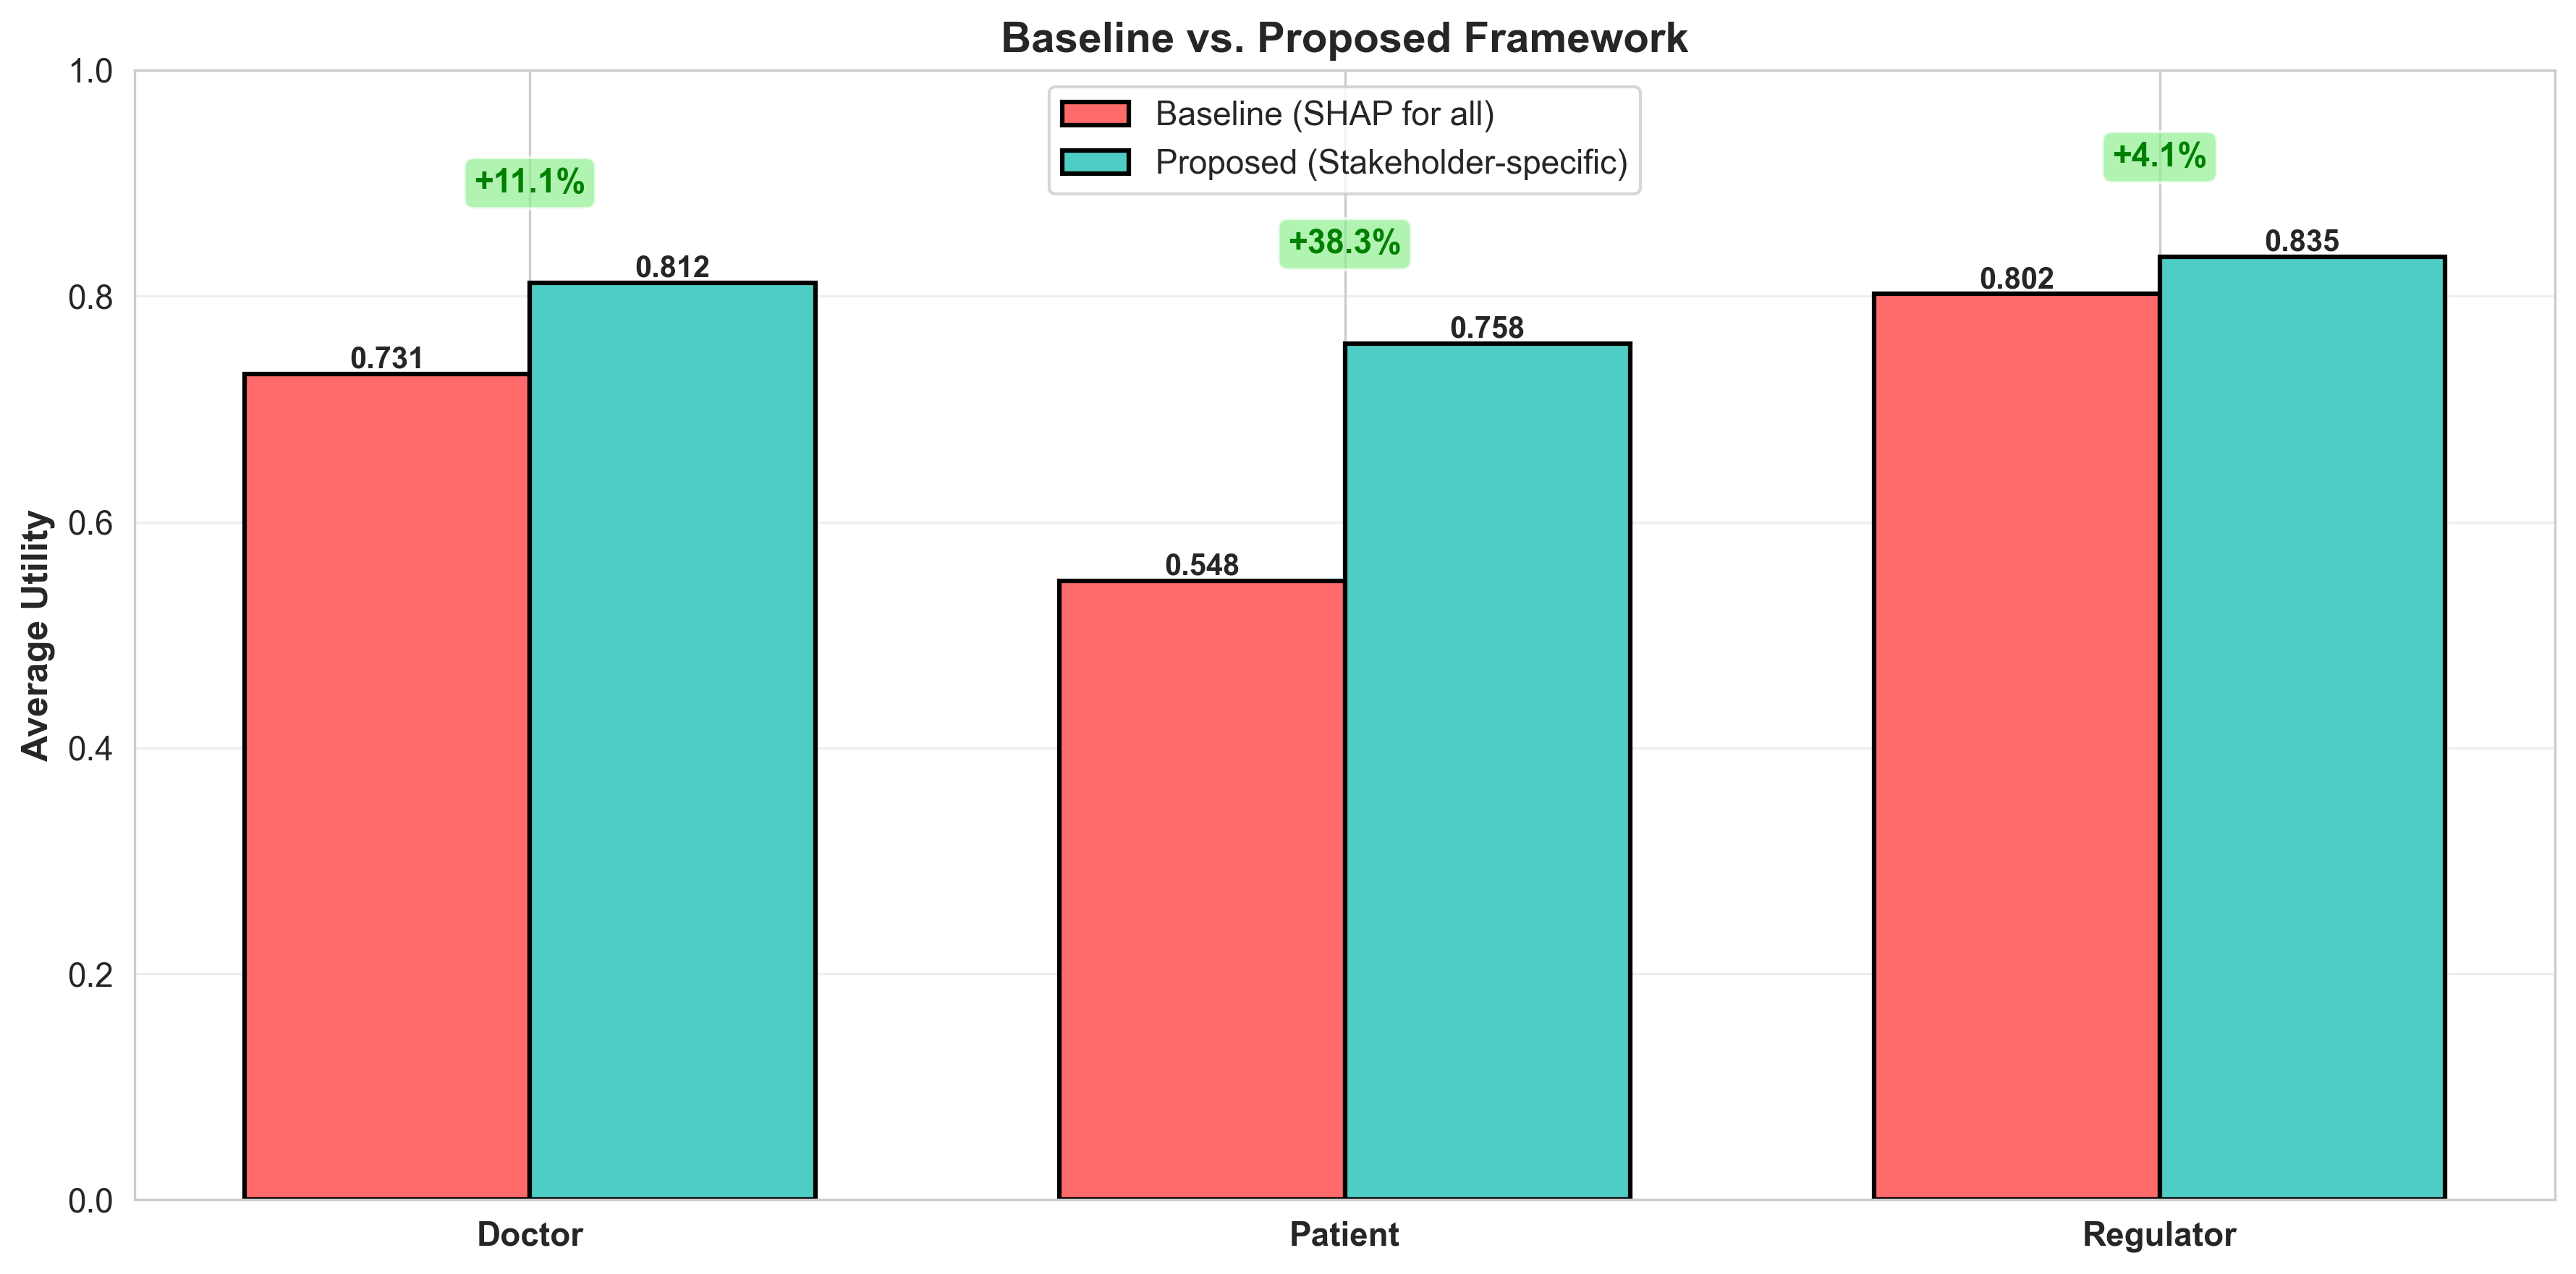
\includegraphics[width=\textwidth]{baseline_vs_proposed.png}
\caption{Average utility for each stakeholder under a static SHAP baseline and under the proposed stakeholder-aware selection policy. The largest improvement is observed for patients, whose explanation needs emphasize interpretability and trust, but all groups benefit from role-specific explanation assignment.}
\label{fig:baseline_vs_proposed}
\end{figure*}

\begin{table}[t]
\centering
\begin{tabular}{lccc}
\toprule
Stakeholder & Baseline Utility & Proposed Utility & Gain \\
\midrule
Doctor & 0.731 & 0.812 & +11.1\% \\
Patient & 0.548 & 0.758 & +38.3\% \\
Regulator & 0.802 & 0.835 & +4.1\% \\
\midrule
Average & 0.694 & 0.801 & +15.4\% \\
\bottomrule
\end{tabular}
\caption{Average utility gains from stakeholder-aware explanation selection compared with a fixed SHAP baseline.}
\label{tab:utility_gain}
\end{table}

This result is important because it suggests that role-aware explanation selection is not only conceptually sound but also practically beneficial. The improvement is largest for patients, whose information needs are often more sensitive to clarity and interpretability. However, even the regulator, whose utility function emphasizes transparency and auditability, benefits from a more tailored explanation policy. This suggests that a fixed, universal explanation strategy is suboptimal even under relatively small evaluation settings.

\section{Limitations and Discussion}

Although the framework demonstrates clear promise, several important limitations must be acknowledged. First, the utility functions are heuristic approximations. Real users have heterogeneous preferences and may update their evaluation of an explanation depending on the decision context, prior trust, and domain expertise. Second, the empirical evaluation is based on a relatively small and controlled dataset, which limits generalization to broader clinical or operational settings. Third, the current study does not include a human-subject validation with real clinicians, patients, and regulators; therefore the results should be interpreted as technical evidence of potential usefulness rather than definitive evidence of real-world impact. Fourth, the framework is currently evaluated on a binary classification setting, and extension to multi-class or multi-label problems remains open. Fifth, generating multiple explanation candidates increases computational cost and may be challenging in real-time deployment settings.

These limitations define the boundary between a promising research framework and a robust operational system. The value of the proposed approach is that it makes stakeholder dependence explicit and provides a principled mechanism for tailoring explanations. However, its deployment would require further validation with real users, governance-informed constraints, and stronger evidence that explanation selection improves actual understanding and decisions rather than merely changing the presentation of model outputs.

\section{Future Work}

Future work should address both methodological and operational challenges. A short-term priority is to conduct human-subject studies to calibrate the utility functions against actual user preferences. This would allow the system to move from expert-designed weights to empirically grounded stakeholder models. Another important direction is to extend the framework to multi-class, multi-label, and temporal decision settings. Real-world applications often involve more complex prediction tasks and numerous stakeholders with interacting objectives. Furthermore, future systems should incorporate fairness constraints and institutional governance requirements into the utility function, making explanation selection suitable for regulated environments.

Longer-term work should also consider the integration of causal reasoning and treatment-effect estimation. In high-stakes settings, the value of an explanation often depends not only on what features drive the prediction, but what interventions would change the outcome or mitigate risk. These directions are essential if the next generation of XAI systems is to support real decisions rather than merely document model predictions.

\section{Conclusion}

This paper argues that explanation quality should not be evaluated solely by model fidelity. In high-stakes settings, the more relevant question is whether an explanation is useful to the stakeholder who must interpret, act on, or regulate a decision. We formalize this perspective as a utility-based explanation-selection problem and show that different stakeholders prefer different explanations for the same model output.

The empirical results support the claim that a one-size-fits-all explanation strategy is suboptimal. By explicitly modeling stakeholder utility and by selecting the explanation that maximizes it, we improve the practical value of XAI systems in decision settings where user goals differ substantially. At the same time, the current framework is best viewed as a foundational step rather than a final operational solution. Real-world deployment would require human validation, richer datasets, stronger fairness and governance safeguards, and a deeper understanding of how explanation choice affects trust, comprehension, and downstream decisions.

The broader implication of this work is straightforward: the next generation of explainable AI systems should be designed not only to explain the model, but also to serve the decision needs of the people who rely on it.

\appendix
\section{Contribution Summary}

This appendix summarizes the novelty and significance of the work in a concise form. The key contribution is the move from model-centric explainability to stakeholder-aware decision utility. Rather than assuming that the most faithful explanation is the best explanation, we treat explanation selection as a decision-theoretic choice problem in which each stakeholder has a different utility function. This framing is novel because it connects explanation quality to decision context, user role, and downstream action. The empirical contribution is equally important: our results show that explanation preferences diverge systematically across doctors, patients, and regulators, and that a role-aware policy outperforms a uniform baseline. In effect, this work argues that explainability should be designed as a user-centered decision support mechanism rather than as a purely technical model-analysis tool.

\section{Repository and Reproducibility}

The code used to generate the results and figures is available in the accompanying project repository. The repository includes the model training pipeline, explanation generators, utility functions, and plotting scripts needed to reproduce the reported results. \textbf{Repository link:} \url{https://github.com/your-org/stakeholder-aware-xai}. If the final submission requires a persistent public repository, the link should be replaced with the corresponding verified project URL before upload.

\bibliographystyle{unsrtnat}
\bibliography{references}

\end{document}
